\documentclass[10pt]{article}
\usepackage[polish]{babel}
\usepackage[utf8]{inputenc}
\usepackage[T1]{fontenc}
\usepackage{amsmath}
\usepackage{amsfonts}
\usepackage{amssymb}
\usepackage[version=4]{mhchem}
\usepackage{stmaryrd}
\usepackage{graphicx}
\usepackage[export]{adjustbox}
\graphicspath{ {./images/} }

\title{GIMNAZJUM }

\author{}
\date{}


\newcommand\Varangle{\mathop{{<\!\!\!\!\!\text{\small)}}\:}\nolimits}

\begin{document}
\maketitle
\begin{enumerate}
  \item Trzęsienie ziemi zniszczyło tarczę zegara na wieży. Jedno pęknięcie biegnie od liczby 11 do liczby 3, drugie łączy liczby 1 i 8 . Oba pęknięcia biegną wzdłuż linii prostych. Jaki kąt tworzą te proste?
  \item Trójkąt ABC podzielono na cztery figury o polach \(S_{1}\), \(S_{2}, S_{3}, S_{4}\) jak na rysunku obok. Czy jest możliwe, by liczby \(S_{1}, S_{2}, S_{3}, S_{4}\) były równe? Odpowiedź uzasadnij.\\
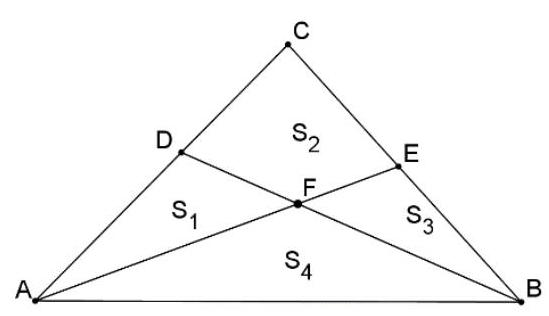
\includegraphics[max width=\textwidth, center]{2024_11_21_15d8c8dfe5a0f4f689ffg-1}
  \item Dla pewnej liczby naturalnej \(n\) ułamek \(\frac{5 n+6}{8 n+7}\) jest skracalny. Przez jaką liczbę?
\end{enumerate}

\section*{LICEUM}
\begin{enumerate}
  \item Udowodnij, że dla liczb rzeczywistych \(a, b, x\) zachodzi nierówność:
\end{enumerate}

\[
|a \sin x+b \cos x| \leq \sqrt{a^{2}+b^{2}}
\]

\begin{enumerate}
  \setcounter{enumi}{1}
  \item W rozgrywkach ligi piłkarskiej wzięło udział \(2 n\) drużyn \((n \geq 2)\) i odbyło się \(2 n-1\) kolejek. W każdej kolejce każda drużyna rozegrała jeden mecz. Dowolne dwie drużyny spotkały się ze sobą podczas rozgrywek w dokładnie jednym meczu. Ponadto w każdym meczu jedna drużyna była gospodarzem, a druga - gościem. Drużynę nazwiemy podróżującą, jeżeli w dowolnych dwóch sąsiednich kolejkach była ona raz gospodarzem i raz gościem. Udowodnić, że istnieją co najwyżej dwie drużyny podróżujące.
  \item Dany jest kwadrat \(A B C D\). Punkt \(P\) leży na półprostej \(A B\) na zewnątrz odcinka \(A B\). Punkt \(Q\) leży na półprostej \(B C\) na zewnątrz odcinka BC, jak na rysunku. Wykaż, że jeśli
\end{enumerate}

\[
A P=P Q+Q C
\]

to \(\Varangle P D Q=45^{\circ}\).\\
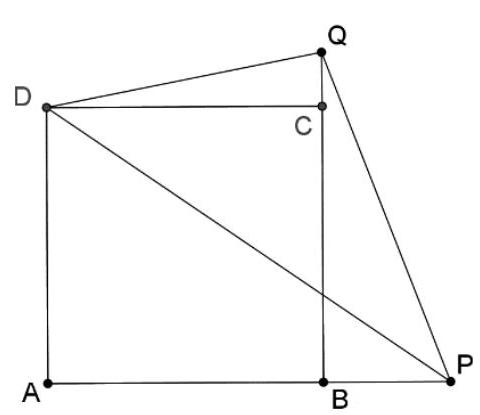
\includegraphics[max width=\textwidth, center]{2024_11_21_15d8c8dfe5a0f4f689ffg-1(1)}


\end{document}